\documentclass[twocolumn]{article}
\usepackage{graphicx}
\usepackage[utf8]{inputenc}
\usepackage[colorlinks = true]{hyperref}
\usepackage[style=authoryear-ibid,backend=biber]{biblatex}

\addbibresource{main.bib}

\title{Individual report on FPGAs and there use in simulating older computer systems}
\author{Harry James Hall}
\date{November 2021}

\begin{document}

\maketitle

\section{Introduction}
\paragraph{FPGA stands for Field Programmable Logic Array.} They are a commercially available device that normally comes in the form of a chip that can be placed on a stand alone device, dev board or something like a PCIe card to be put into a Desktop Computer, Server, or Workstation. They have been used in a wide variety of devices including routers, cellular base stations, and high-speed cameras.

\paragraph{}FPGAs are a device that can be used to simulate a large number of digital circuits and systems without having to go through the complexities and cost of manufacturing custom silicon. This includes making things like CPUs \autocite{hardesty_2012}, ASICs, and even glue logic.

\paragraph{}Our project involves simulating an older non-standard computer system using an FPGA. FPGAs are useful for this as they can simulate a wide range of electronic devices within themselves and do so with both high accuracy and performance. Software based solutions don't normally have the accuracy and performance that FPGAs offer without using hardware that is vastly more powerful than the system being simulated. This makes them better at simulating older devices like this than a purely software based approach.

\section{Background}
\subsection{What's inside an FPGA}
\paragraph{}An FPGA contains various logic elements such as Memory cells, programmable interconnects, DSPs, lookup tables\autocite{vaughn}, and other components. Lookup tables can act as combinatorial logic \autocite{moore_2019} and when combined with the other elements in an FPGA they can be used to simulate a wide variety of digital logic circuitry. In order for all this to work these components have to be programmable. This is typically done using SRAM latches \cite{vaughn} to hold programming information. Since this type of memory is volatile it normally has to be reprogrammed on startup from a secondary store such as NAND or EEPROM. This comes with the advantage that many FPGAs can be reprogrammed on the fly while in operation. All of this stuff together is called Programmable Logic.

\paragraph{}FPGAs also have things like IO blocks to communicate with other components such as DRAM, a PCIe host, USB, Ethernet, or digital components. Many FPGAs also come with things like CPUs built in, these chips are full SoCs rather than just FPGAs as they contain more than just programmable logic.

\paragraph{}The group will most likely be working with an FPGA SoC containing an ARM CPU. Interestingly FPGAs can also simulate CPUs as I myself have experimented with. It saves programmable logic resources for other tasks if the CPU is implemented in hardware and also often means the CPU can be faster and more efficient than what programmable logic can do on it's own. We most likely won't be using the CPU to emulate the Sharp chip as they have completely different ISAs \autocite{realboy-emulator}\autocite{ARMISA}. It might however be useful for our stretch goal which involves emulating a system with an ARM7TDMI chip as it's instruction set is more similar to that used in commodity ARM-based SoCs. It could also be useful for communicating with external devices like monitors or controller input.

\begin{figure}[h]
\label{inside FPGA}
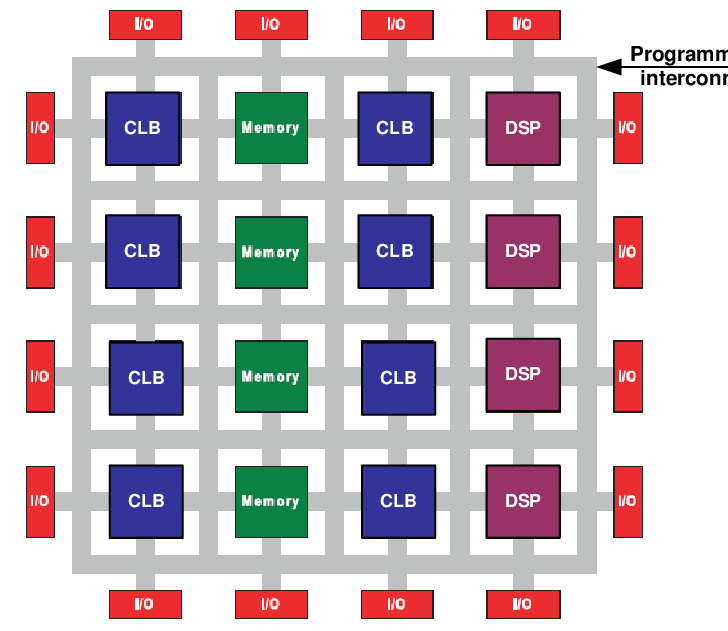
\includegraphics[scale=0.9]{FPGA insides 1.png}
\caption{Inside a simple FPGA}
\end{figure}

In Figure 1  CLB stands for Complex Logic Block. DSP is Digital Signal Processor.

\subsection{Using FPGAs for simulating older computer systems}
\paragraph{}FPGAs are useful because they approach hardware level emulation without having to really manufacture the chips that older systems used. This is good because many of these chips are discontinued. You would also have to buy a separate device for each device you want to simulate whereas with an FPGA they can run a wide variety of images on a single device - although often not simultaneously.

\subsection{Existing FPGA simulation  projects}
\paragraph{Multiple projects to simulate older computer and gaming systems using an FPGA or programmable logic device already exist.} In this section I outline some of these. Many of these projects are made by hobbyists and are open source. Some like the J-core open processor have commercial applications.

\paragraph{}FPGAs from both Altera/Intel and Xilinx have been used for these projects. I myself have experimented with the J-core processor for a brief time using a Xilinx Spartan-6 chip. This project simulates the SuperH 2 processor from Hitachi with some custom extensions. The patents on this ISA have expired which is why they are able to attempt this project legally. \autocite{j-core-open-processor} There are versions of the Linux Kernel and Linux based OSes that can run on this processor.

\paragraph{}It's also possible to implement more modern instruction sets using an FPGA such as RISC-V. RISC-V is an open source ISA so is perfect for implementation in Open Source projects. You can find one of these called VexRiscv here:\href{https://github.com/SpinalHDL/VexRiscv}{VexRiscv}. This one is actually independent of any particular FPGA and can run on chips made by different companies.

\subsubsection{Hardware projects}
\begin{itemize}
    \item MiSTer FPGA project
    \item Analogue Pocket
\end{itemize}

In the MiSTer FPGA project an SoC with a built in dual core ARM Cortex-A9 processor as well as programmable logic\autocite{terrasic} is used. This SoC is built into a Dev board called the Terrasic DE10-Nano \autocite{mister}. The ARM cores are responsible for programming different images onto the FPGA/Programmable Logic component in the SoC.

\subsubsection{Firmware images}
\begin{itemize}
    \item \href{https://boogermann.github.io/Bible_MiSTer/core-status/}{Cores for the MiSTer project}
    \item \href{https://hackaday.com/2019/03/23/game-boy-recreated-in-verilog/}{VerilogBoy article}
    \item \href{https://j-core.org/}{J-core open processor}
\end{itemize}



\section{Acronyms}
\paragraph{FPGA} Field Programmable Grid Array
\paragraph{ISA} Instruction Set Architecture
\paragraph{CPU} Central Processing Unit
\paragraph{ALU} Arithmetic and Logic Block
\paragraph{ASIC} Application Specific Integrated Circuit
\paragraph{SoC} System On a Chip
\paragraph{LE} Logic Element

\printbibliography

\end{document}
